\section{Results}\label{sec:results}

\subsection{Functional verification}
For all 80 training runs, the executed Mapping~S program reproduced the reference prediction on each of the first 1,500 test samples.
The executed Mapping~C program, followed by the vote reduction in NumPy, reproduced it on each of the first 200 test samples.
The compile-time simplification of Section~\ref{sec:norm} is exact by construction, and these checks confirm it on every model.
Conflicting literals do occur in FPTM. For example, 32 of the 46 clauses of the seed-0 2-clause NSL-KDD model include some feature both plainly and negated.

\subsection{Accuracy and model size}\label{sec:accuracy}
Table~\ref{tab:accuracy} lists validation and test accuracy, the number of included literals and the model size.
The model size assumes a sparse encoding with one feature index and one polarity bit per included literal.
Values are the mean and standard deviation over seeds.

\begin{table}[!htbp]
\small
\centering
\caption{Accuracy and model size, mean $\pm$ standard deviation over seeds (Table~\ref{tab:hyper}). Test accuracy is that of the exported clause set at the epoch with the best validation accuracy. Literals: included literals over all clauses. Strict: FPTM trainer with $\LF=1$.}
\label{tab:accuracy}
\begin{tabular}{lrrrrr}
\toprule
Model & Cl./class & Val.\ acc.\ (\%) & Test acc.\ (\%) & Literals & Size (KiB) \\
\midrule
\multicolumn{6}{l}{\textit{WOS-46985}} \\
FPTM & 2 & 81.64 $\pm$ 0.55 & 81.98 $\pm$ 0.45 & 16,466 & 30.2 \\
FPTM & 10 & 86.46 $\pm$ 0.25 & 85.96 $\pm$ 0.06 & 56,163 & 102.8 \\
FPTM & 20 & 87.91 $\pm$ 0.23 & 87.82 $\pm$ 0.33 & 59,753 & 109.4 \\
FPTM & 40 & 88.44 $\pm$ 0.20 & 88.09 $\pm$ 0.04 & 92,907 & 170.1 \\
FPTM & 100 & 89.62 $\pm$ 0.15 & 89.50 $\pm$ 0.01 & 150,218 & 275.1 \\
Strict & 200 & 90.49 $\pm$ 0.06 & 90.87 $\pm$ 0.09 & 103,091 & 188.8 \\
Strict & 400 & 90.53 $\pm$ 0.14 & 90.87 $\pm$ 0.09 & 183,056 & 335.2 \\
Vanilla TM & 400 & 78.27 & 78.26 & 2,984,562 & 5,464.9 \\
\midrule
\multicolumn{6}{l}{\textit{ALeRCE}} \\
FPTM & 2 & 90.55 $\pm$ 0.35 & 90.54 $\pm$ 0.29 & 2,561 & 3.8 \\
FPTM & 10 & 92.90 $\pm$ 0.11 & 92.84 $\pm$ 0.14 & 10,537 & 15.4 \\
FPTM & 20 & 93.26 $\pm$ 0.05 & 93.23 $\pm$ 0.10 & 11,776 & 17.2 \\
FPTM & 40 & 93.76 $\pm$ 0.07 & 93.65 $\pm$ 0.04 & 19,011 & 27.8 \\
FPTM & 100 & 93.77 $\pm$ 0.06 & 93.59 $\pm$ 0.06 & 33,623 & 49.3 \\
Strict & 200 & 90.81 $\pm$ 0.08 & 90.92 $\pm$ 0.14 & 50,933 & 74.6 \\
Strict & 400 & 91.80 $\pm$ 0.07 & 92.12 $\pm$ 0.14 & 105,409 & 154.4 \\
Strict & 600 & 92.42 $\pm$ 0.08 & 92.63 $\pm$ 0.08 & 160,015 & 234.4 \\
Strict & 1,000 & 93.13 & 93.28 & 273,580 & 400.8 \\
Vanilla TM & 200 & 78.80 $\pm$ 0.42 & 78.65 $\pm$ 0.55 & 314,385 & 460.5 \\
Vanilla TM & 1,000 & 91.53 & 91.43 & 912,839 & 1,337.2 \\
\midrule
\multicolumn{6}{l}{\textit{NSL-KDD}} \\
FPTM & 2 & 96.19 $\pm$ 0.56 & 84.11 $\pm$ 0.26 & 3,838 & 4.2 \\
FPTM & 10 & 98.23 $\pm$ 0.04 & 85.63 $\pm$ 0.14 & 15,595 & 17.1 \\
FPTM & 20 & 98.62 $\pm$ 0.06 & 85.94 $\pm$ 0.22 & 18,117 & 19.9 \\
FPTM & 40 & 98.74 $\pm$ 0.04 & 86.40 $\pm$ 0.02 & 34,685 & 38.1 \\
FPTM & 100 & 98.79 $\pm$ 0.00 & 86.26 $\pm$ 0.01 & 69,400 & 76.2 \\
Strict & 200 & 98.54 $\pm$ 0.04 & 85.82 $\pm$ 0.07 & 91,111 & 100.1 \\
Strict & 400 & 98.71 $\pm$ 0.07 & 86.12 $\pm$ 0.18 & 216,928 & 238.3 \\
Strict & 600 & 98.79 $\pm$ 0.03 & 86.23 $\pm$ 0.06 & 348,593 & 383.0 \\
Strict & 1,000 & 98.91 & 86.02 & 436,996 & 480.1 \\
Vanilla TM & 200 & 93.23 $\pm$ 0.83 & 81.22 $\pm$ 2.18 & 407,988 & 448.2 \\
Vanilla TM & 1,000 & 98.21 & 86.08 & 1,385,591 & 1,522.3 \\
\bottomrule
\end{tabular}

\end{table}

On ALeRCE, FPTM reaches 90.54\% $\pm$ 0.29\% with 2 clauses per class and 93.23\% $\pm$ 0.10\% with 20 clauses per class.
The strict $\LF=1$ models need 1,000 clauses per class for 93.28\%. With 600 clauses per class they reach 92.63\% $\pm$ 0.08\%.
The 20-clause FPTM uses 11,776 literals on average, $13.6\times$ fewer than the 600-clause $\LF=1$ model (160,015).
The vanilla TM reaches 78.65\% $\pm$ 0.55\% with 200 and 91.43\% with 1,000 clauses per class.

On NSL-KDD, all models trained with the FPTM trainer and at least 10 clauses per class lie between 85.63\% and 86.40\% test accuracy.
The validation accuracy of the same models lies between 98.23\% and 98.91\%. Validation and test rankings do not agree, because KDDTest+ differs in distribution from the training data.
Test differences below about 0.5 points on NSL-KDD should therefore not be read as a ranking.
The vanilla TM reaches 81.22\% $\pm$ 2.18\% with 200 and 86.08\% with 1,000 clauses per class.

On WOS-46985, the strict $\LF=1$ models reach the highest accuracy, 90.87\% $\pm$ 0.09\% with both 200 and 400 clauses per class.
FPTM improves with the clause count, from 81.98\% $\pm$ 0.45\% with 2 clauses to 89.50\% $\pm$ 0.01\% with 100 clauses per class.
FPTM clauses on WOS are long. With the hyperparameters of Table~\ref{tab:hyper}, the 2-clause models carry about 1,050 to 1,300 literals per clause, mostly negated word literals.
The vanilla TM with 400 clauses per class reaches 78.26\% (one seed).
No hyperparameter search was performed for the vanilla TM on any dataset. Its results should not be read as the capability of the vanilla TM.

\subsection{Predicted 7~nm \gainp{} cost, Mapping~S}
Table~\ref{tab:mapS} gives the program length, the batch latency, the energy per sample and the throughput per unit area for Mapping~S at the two predicted 7~nm corners.
\wosnew{Fig.~\supref{fig:paretofull} of the supplementary material plots test accuracy against energy per sample at the optimistic corner for all three datasets.}
The cycle count is a property of the program and does not depend on the process. It varies between seeds because the trained clauses differ.

\begin{sidewaystable}
\footnotesize
\setlength{\tabcolsep}{4pt}
\centering
\caption{Mapping~S (sample-stationary) at the predicted 7~nm corners, mean $\pm$ standard deviation over seeds where shown. Rows/col.: CAM rows per logical column. Subarrays: stacked subarrays per logical column. Latency includes refresh. Energy includes dynamic, refresh, gain-cell static and controller energy (M6). It excludes input loading (M4) and model-SRAM leakage (M7). Throughput includes input loading and is given per mm$^2$ of occupied subarrays and model SRAM (M7) of a 256-subarray macro.}
\label{tab:mapS}
\begin{tabular}{lrrrrrrrr}
\toprule
\multirow{2}{*}{Model (cl./class)} & Rows & Sub- & Cycles & \multicolumn{2}{c}{Batch latency ($\mu$s)} & \multicolumn{2}{c}{Energy (nJ/sample)} & Thr., opt. \\
 & /col. & arrays & ($\times10^3$) & cons. & opt. & cons. & opt. & (M/s/mm$^2$) \\
\midrule
\multicolumn{9}{l}{\textit{WOS-46985}} \\
FPTM (2) & 10,060 & 79 & 729.6 $\pm$ 86.5 & \hyp{1,096} & \hyp{737} & \hyp{35.06 $\pm$ 4.15} & \hyp{9.871 $\pm$ 1.168} & \hyp{1.43} \\
FPTM (10) & 10,083 & 79 & 2,370.7 $\pm$ 200.0 & \hyp{3,562} & \hyp{2,394} & \hyp{112.41 $\pm$ 9.72} & \hyp{31.936 $\pm$ 2.715} & \hyp{0.392} \\
FPTM (20) & 10,064 & 79 & 1,404.3 $\pm$ 73.0 & \hyp{2,110} & \hyp{1,418} & \hyp{64.42 $\pm$ 3.34} & \hyp{18.800 $\pm$ 0.976} & \hyp{0.650} \\
FPTM (40) & 10,068 & 79 & 2,196.5 $\pm$ 383.9 & \hyp{3,301} & \hyp{2,218} & \hyp{100.81 $\pm$ 17.58} & \hyp{29.409 $\pm$ 5.135} & \hyp{0.390} \\
FPTM (100) & 10,048 & 79 & 1,821.2 $\pm$ 202.8 & \hyp{2,737} & \hyp{1,839} & \hyp{83.73 $\pm$ 9.31} & \hyp{24.665 $\pm$ 2.747} & \hyp{0.405} \\
Strict (200) & 10,037 & 79 & 41.5 $\pm$ 0.0 & \hyp{62.4} & \hyp{41.9} & \hyp{3.77 $\pm$ 0.02} & \hyp{1.110 $\pm$ 0.006} & \hyp{15.9} \\
Strict (400) & 10,041 & 79 & 95.7 $\pm$ 0.0 & \hyp{144} & \hyp{96.7} & \hyp{7.74 $\pm$ 0.31} & \hyp{2.267 $\pm$ 0.094} & \hyp{6.44} \\
Vanilla TM (400) & 10,041 & 79 & 95.7 & \hyp{144} & \hyp{96.6} & \hyp{56.34} & \hyp{17.161} & \hyp{0.951} \\
\midrule
\multicolumn{9}{l}{\textit{ALeRCE}} \\
FPTM (2) & 1,231 & 10 & 70.3 $\pm$ 4.0 & \hyp{106} & \hyp{71.0} & \hyp{1.19 $\pm$ 0.07} & \hyp{0.192 $\pm$ 0.011} & \hyp{121} \\
FPTM (10) & 1,233 & 10 & 276.1 $\pm$ 8.6 & \hyp{415} & \hyp{279} & \hyp{4.65 $\pm$ 0.14} & \hyp{0.754 $\pm$ 0.024} & \hyp{30.4} \\
FPTM (20) & 1,237 & 10 & 270.1 $\pm$ 10.0 & \hyp{406} & \hyp{273} & \hyp{4.42 $\pm$ 0.14} & \hyp{0.726 $\pm$ 0.025} & \hyp{30.9} \\
FPTM (40) & 1,241 & 10 & 423.2 $\pm$ 37.9 & \hyp{636} & \hyp{427} & \hyp{6.84 $\pm$ 0.55} & \hyp{1.129 $\pm$ 0.095} & \hyp{19.4} \\
FPTM (100) & 1,221 & 10 & 457.1 $\pm$ 22.0 & \hyp{687} & \hyp{462} & \hyp{6.73 $\pm$ 0.31} & \hyp{1.161 $\pm$ 0.055} & \hyp{17.1} \\
Strict (200) & 1,210 & 10 & 89.0 $\pm$ 0.0 & \hyp{134} & \hyp{89.9} & \hyp{1.90 $\pm$ 0.00} & \hyp{0.304 $\pm$ 0.000} & \hyp{82.4} \\
Strict (400) & 1,214 & 10 & 205.3 $\pm$ 0.0 & \hyp{308} & \hyp{207} & \hyp{4.28 $\pm$ 0.01} & \hyp{0.686 $\pm$ 0.001} & \hyp{31.2} \\
Strict (600) & 1,218 & 10 & 332.3 $\pm$ 0.0 & \hyp{499} & \hyp{335} & \hyp{6.84 $\pm$ 0.02} & \hyp{1.098 $\pm$ 0.003} & \hyp{17.0} \\
Strict (1,000) & 1,218 & 10 & 602.3 & \hyp{905} & \hyp{608} & \hyp{12.27} & \hyp{1.969} & \hyp{7.54} \\
Vanilla TM (200) & 1,210 & 10 & 88.9 $\pm$ 0.0 & \hyp{134} & \hyp{89.7} & \hyp{4.23 $\pm$ 0.45} & \hyp{0.648 $\pm$ 0.066} & \hyp{48.4} \\
Vanilla TM (1,000) & 1,218 & 10 & 600.7 & \hyp{903} & \hyp{606} & \hyp{17.90} & \hyp{2.800} & \hyp{3.67} \\
\midrule
\multicolumn{9}{l}{\textit{NSL-KDD}} \\
FPTM (2) & 237 & 2 & 96.5 $\pm$ 0.4 & \hyp{145} & \hyp{97.5} & \hyp{1.29 $\pm$ 0.00} & \hyp{0.147 $\pm$ 0.001} & \hyp{445} \\
FPTM (10) & 243 & 2 & 387.3 $\pm$ 6.6 & \hyp{582} & \hyp{391} & \hyp{5.15 $\pm$ 0.09} & \hyp{0.589 $\pm$ 0.010} & \hyp{107} \\
FPTM (20) & 244 & 2 & 403.3 $\pm$ 24.9 & \hyp{606} & \hyp{407} & \hyp{5.05 $\pm$ 0.26} & \hyp{0.583 $\pm$ 0.031} & \hyp{102} \\
FPTM (40) & 248 & 2 & 741.4 $\pm$ 140.4 & \hyp{1,114} & \hyp{749} & \hyp{8.96 $\pm$ 1.47} & \hyp{1.039 $\pm$ 0.174} & \hyp{54.5} \\
FPTM (100) & 228 & 2 & 911.6 $\pm$ 57.5 & \hyp{1,370} & \hyp{920} & \hyp{10.03 $\pm$ 0.60} & \hyp{1.184 $\pm$ 0.072} & \hyp{39.2} \\
Strict (200) & 217 & 2 & 136.6 $\pm$ 0.0 & \hyp{205} & \hyp{138} & \hyp{2.46 $\pm$ 0.07} & \hyp{0.279 $\pm$ 0.008} & \hyp{246} \\
Strict (400) & 221 & 2 & 314.7 $\pm$ 0.1 & \hyp{473} & \hyp{318} & \hyp{5.74 $\pm$ 0.47} & \hyp{0.650 $\pm$ 0.051} & \hyp{81.9} \\
Strict (600) & 225 & 2 & 509.5 $\pm$ 0.0 & \hyp{766} & \hyp{514} & \hyp{9.28 $\pm$ 0.64} & \hyp{1.051 $\pm$ 0.070} & \hyp{40.6} \\
Strict (1,000) & 225 & 2 & 923.0 & \hyp{1,387} & \hyp{932} & \hyp{15.29} & \hyp{1.738} & \hyp{19.5} \\
Vanilla TM (200) & 217 & 2 & 136.5 $\pm$ 0.1 & \hyp{205} & \hyp{138} & \hyp{4.97 $\pm$ 0.07} & \hyp{0.553 $\pm$ 0.007} & \hyp{140} \\
Vanilla TM (1,000) & 225 & 2 & 922.0 & \hyp{1,386} & \hyp{931} & \hyp{22.80} & \hyp{2.558} & \hyp{8.82} \\
\bottomrule
\end{tabular}

\end{sidewaystable}


A strict clause costs one COMPARE whatever its length.
A fuzzy clause costs a miss count that grows with its length.
The trade-off is therefore decided by how many strict clauses an FPTM clause replaces.

On ALeRCE, above about 92.5\% accuracy, FPTM is more accurate and needs fewer cycles and less predicted energy.
The 20-clause FPTM (93.23\%) needs 270.1k cycles and \hyp{4.42~nJ (conservative) or 0.73~nJ (optimistic)} per sample, including the controller.
The 600-clause $\LF=1$ model (92.63\%) needs 332.3k cycles and \hyp{6.84~nJ or 1.10~nJ}.
The 40-clause FPTM (93.65\%) needs 423.2k cycles and \hyp{6.84~nJ or 1.13~nJ}. The 1,000-clause $\LF=1$ model (93.28\%) needs 602.3k cycles and \hyp{12.27~nJ or 1.97~nJ}.
At the low end, the 200-clause $\LF=1$ model is 0.38 points more accurate on average than the 2-clause FPTM, about 1.3 standard deviations of the FPTM runs. It needs $1.27\times$ more cycles and \hyp{$1.6\times$} more energy.

On NSL-KDD, at moderate accuracy, the strict models need fewer cycles and less predicted energy.
The 200-clause $\LF=1$ model (85.82\%) needs 136.6k cycles and \hyp{2.46~nJ or 0.28~nJ}, against 403.3k cycles and \hyp{5.05~nJ or 0.58~nJ} for the 20-clause FPTM (85.94\%).
At the top of the accuracy range, the 40-clause FPTM (86.40\%) and the 600-clause $\LF=1$ model (86.23\%) need similar predicted energy. At the conservative corner, they need \hyp{8.96~nJ and 9.28~nJ}, although the FPTM needs more cycles.

On WOS-46985, the strict model is more accurate and needs fewer cycles and less predicted energy.
The 200-clause $\LF=1$ model needs 41.5k cycles and \hyp{3.77~nJ or 1.11~nJ} for 90.87\%.
The 100-clause FPTM needs 1,821k cycles and \hyp{83.7~nJ or 24.7~nJ} for 89.50\%.
Long FPTM clauses make the miss counts expensive. The 10,000-bit inputs also need 79 stacked subarrays per logical column, which raises the predicted static energy and lowers the predicted throughput density. \hyp{Only three such stacks fit in a 256-subarray macro, so the controller energy is shared by fewer samples.}

\subsection{Predicted 7~nm \gainp{} cost, Mapping~C}\label{sec:mapCres}
\wosnew{Table~\supref{tab:mapC} of the supplementary material reports Mapping~C in full.}
Here a strict model evaluates all its clauses in one COMPARE, one WRITE and one READ, i.e., 3 cycles.
Its area, however, grows with the clause count. The 1,000-clause $\LF=1$ ALeRCE model needs 15,000 clause columns and \hyp{1.71~mm$^2$}.
Its 15,000 clause outputs must also be reduced outside the array.
The 20-clause FPTM fits in \hyp{0.036~mm$^2$} and leaves 300 values to reduce, but needs 30,258 cycles per sample because the miss count is built feature by feature.
\wosnew{The 20-clause FPTM needs} \hyp{222~nJ or 65.9~nJ} \wosnew{per sample, against} \hyp{136~nJ or 13.4~nJ} \wosnew{for the 1,000-clause strict model.}
Per sample, Mapping~C needs more predicted energy than Mapping~S for every FPTM and strict model. Each sample activates the whole model array, and the controller energy is not shared between samples.


\subsection{Comparison with CPU inference and TM hardware}\label{sec:compare}
To our knowledge, no hardware implementation of FPTM has been reported. The FPTM paper reports CPU inference only~\cite{hnilov2025fptm}.
We therefore compare \gainp{} with FPTM and TM inference on a CPU, and with published hardware accelerators for the vanilla TM and other TM variants.

\paragraph{CPU}
We ran every exported model on the CPU of our environment, an Intel Xeon processor at 2.10~GHz in a virtual machine.
\wosnew{The virtual machine exposes no power counters, so we bound the CPU energy from below by assuming that the active core draws at least 1~W.}
\hyp{For this comparison, the \gainp{} energy includes input loading (M4), because the CPU time includes input packing. Under this bound, the fastest single-thread CPU kernel needs between $63\times$ and about $7{,}100\times$ more energy per classification than the predicted \gainp{} at the conservative corner, for every model. For the 20-clause ALeRCE FPTM, the ratio is about $810\times$.}
\wosnew{Section~\supref{cpu} of the supplementary material gives the CPU times, the kernels and the timing protocol.}

\paragraph{TM hardware accelerators}
Table~\ref{tab:tmhw} lists published TM accelerators that report energy or throughput, together with representative \gainp{} predictions.
The comparison is not like for like. The designs differ in dataset, TM variant, model size and technology node, and several of them report simulated rather than measured results.
Our \gainp{} values are predictions for 7~nm. Their energy includes the controller and excludes feature extraction, off-chip input transfer and input loading into the array. Their throughput includes input loading.
\hyp{Over all 30 configurations in Mapping~S and both corners, the predicted \gainp{} energy per classification is 0.15 to 112~nJ, excluding model-SRAM leakage (M7).} The reported TM ASICs and in-memory designs span 30.6~pJ to 191~nJ, and the reported FPGA accelerators 0.6 to 73.6~$\mu$J. \hyp{The predicted \gainp{} energy thus lies within the first range. It is at least $5.3\times$ below the FPGA accelerators, and at least $33\times$ below them for the four listed models.
The occupied subarrays of one 256-subarray macro and its model SRAM take 0.19 to 0.72~mm$^2$, without the sequencer logic. The macro is predicted to classify $1.8\times10^6$ to $4.0\times10^7$ samples per second for the listed models.} The 65~nm ASIC of~\cite{tunheim2026asic} classifies $6.03\times10^4$ samples per second in 2.7~mm$^2$.

\begin{sidewaystable}
\footnotesize
\setlength{\tabcolsep}{4pt}
\centering
\caption{Published TM inference hardware and predicted 7~nm \gainp{}. Energy and throughput as reported by each design. n/r: not reported. Model: TM variant, with clauses per class in parentheses. For \gainp{}, energy includes the controller, excludes input loading and model-SRAM leakage, and is given at the conservative and optimistic corners. Throughput is given at the conservative corner for one 256-subarray macro, with its area including the model SRAM.}
\label{tab:tmhw}
\scriptsize
\setlength{\tabcolsep}{3pt}
\begin{tabular}{>{\raggedright\arraybackslash}p{3.0cm}>{\raggedright\arraybackslash}p{3.2cm}>{\raggedright\arraybackslash}p{2.7cm}>{\raggedright\arraybackslash}p{2.4cm}r>{\raggedright\arraybackslash}p{2.4cm}>{\raggedright\arraybackslash}p{2.9cm}}
\toprule
Design & Platform & Model & Dataset & Acc.\ (\%) & Energy/classif. & Classif./s \\
\midrule
Wheeldon et al.~\cite{wheeldon2020learning} & ASIC, 65~nm, layout & Vanilla TM (20) & Iris & n/r$^{a}$ & 30.6~pJ & n/r \\
Tunheim et al.~\cite{tunheim2026asic} & ASIC, 65~nm, silicon & ConvCoTM & MNIST & 97.42 & 8.6~nJ$^{b}$ & 60.3k (2.7~mm$^2$) \\
Lin et al.~\cite{lin2025tsetlinkws}$^{c}$ & ASIC, 65~nm & CTM & GSCD-12$^{d}$ & 87.35 & 191~nJ$^{e}$ & n/r$^{f}$ \\
Tunheim et al.~\cite{tunheim2023ctm} & FPGA, XC7Z020 & CTM & 2-D Noisy XOR & 99.9 & 0.6~$\mu$J & 4.4M \\
Tunheim et al.~\cite{tunheim2025fpga} & FPGA, XCZU7 & ConvCoTM & MNIST & 97.6 & 13.3~$\mu$J & 134k \\
Mao et al.~\cite{mao2025dtm} & FPGA, ZU7EV & Vanilla TM, CoTM & MNIST & 97.74 & 73.6~$\mu$J$^{g}$ & 22.4k \\
Ghazal et al.~\cite{ghazal2023imbue} & ReRAM IMC, 65~nm$^{h}$ & Vanilla TM & MNIST & 96.48 & 13.9~nJ & n/r \\
Ghazal et al.~\cite{ghazal2023imbue} & ReRAM IMC, 65~nm$^{h}$ & Vanilla TM & KWS-6 & 87.1 & 5.91~nJ & n/r \\
Ghazal et al.~\cite{ghazal2025impact} & Y-Flash IMC, 180~nm$^{h}$ & CoTM & MNIST & 96.3 & 84.2~pJ$^{i}$ & n/r \\
Hnilov~\cite{hnilov2025fptm} & CPU, 16 cores & FPTM (1) & IMDb & n/r$^{j}$ & n/r & 34.5M \\
This work & CPU, 1 thread & FPTM (20) & ALeRCE & 93.23 & not measured & 277k \\
\midrule
This work & \hyp{\gainp{}, 7~nm, pred.} & FPTM (20) & ALeRCE & 93.23 & \hyp{4.42 / 0.73~nJ} & \hyp{3.9M (0.19~mm$^2$)} \\
This work & \hyp{\gainp{}, 7~nm, pred.} & Vanilla TM (1,000) & ALeRCE & 91.43 & \hyp{17.90 / 2.80~nJ} & \hyp{1.8M (0.72~mm$^2$)} \\
This work & \hyp{\gainp{}, 7~nm, pred.} & Strict (200) & NSL-KDD & 85.82 & \hyp{2.46 / 0.28~nJ} & \hyp{39.9M (0.24~mm$^2$)} \\
This work & \hyp{\gainp{}, 7~nm, pred.} & FPTM (20) & NSL-KDD & 85.94 & \hyp{5.05 / 0.58~nJ} & \hyp{13.5M (0.20~mm$^2$)} \\
\bottomrule
\end{tabular}


\vspace{4pt}
\parbox{0.95\textwidth}{\raggedright $^{a}$The reported ASIC accuracy, 97.0\%, is for 100 clauses per class. The energy is for the 20-clause-per-class layout. $^{b}$Accelerator core energy, IO power excluded. $^{c}$Preprint. $^{d}$Google Speech Commands, 12 keywords. $^{e}$Inference core energy normalized to 65~nm. $^{f}$Reported latency 16~ms per inference. $^{g}$Reported IP power times reported latency, as tabulated in~\cite{tunheim2026asic}. $^{h}$Simulation. $^{i}$Sum of the reported clause (67.99~pJ) and class (16.22~pJ) crossbar tile energies per data point. $^{j}$Throughput benchmark of a 1-clause-per-class IMDb model on all cores of an AMD Ryzen 9 7950X3D. The accuracy is not tied to the benchmark.}
\end{sidewaystable}

\subsection{Sensitivity}\label{sec:sens}
We test how the \wosnew{accuracy-oriented} ALeRCE comparison, the 20-clause FPTM against the 600-clause $\LF=1$ model, depends on the modelling choices.
\wosnew{The strict model needs \hyp{1.28$\times$} to \hyp{1.55$\times$} the energy of the FPTM model in every case tested.
The cases are the 16~nm reference points, both predicted 7~nm corners, a per-column energy model, no controller, a five times lower sequencer energy and a 64-subarray macro.
The controller share of the Mapping~S energy is \hyp{3\% to 84\%}, highest on WOS-46985.
With a $10\times$ shorter retention time, the refresh overhead of the FPTM batch latency rises to \hyp{14.3\%} at the conservative corner.
If refresh used the shared sense amplifier instead of lockstep local refresh, Mapping~S on WOS-46985 would not be feasible at the conservative corner, while the ALeRCE ranking would not change.
Section~\\supref{sens} of the supplementary material gives the full analysis.}


\subsection{Accuracy and energy with energy-oriented hyperparameters}\label{sec:energyhp}
\wosnew{The preceding subsections use the accuracy-oriented hyperparameters. This section adds the energy-oriented ones (Section~\ref{sec:method}).
Table~\ref{tab:energyhp} lists the results. Fig.~\ref{fig:front} places both sets of ALeRCE and NSL-KDD models in one accuracy and energy plane.
All energy-oriented models passed the bit-exact check of Section~\ref{sec:method} in both mappings.
On ALeRCE, the two runs differ by at most 0.18 points in accuracy and 14\% in energy.
Both runs share the sample order, so this spread may understate the seed variance (Section~\ref{sec:method}).}

\wosnew{The energy-oriented FPTM models have fewer included literals and a smaller $\LF$. Both shorten the miss counts of Mapping~S.
Their predicted energy falls by $1.6\times$ to $3.7\times$ on ALeRCE and by $3.1\times$ to $12\times$ on NSL-KDD, at both corners.
The FPTM accuracy changes by $-0.30$ to $+1.78$ points on these two datasets.
The energy-oriented strict models of these two datasets need 2\% to 13\% less predicted energy at the same cycle count, because their clauses are shorter. On ALeRCE, they also gain 0.8 to 3.1 points of accuracy.
The 200-clause strict model gains 3.06 points. This gain comes mainly from the hyperparameters, not from the longer schedule: its validation accuracy already reaches 93.85\% within 50 epochs, against 90.81\% with the accuracy-oriented settings.}

\wosnew{A model lies on the accuracy and energy front when no other model of the same dataset dominates it. A model dominates another when it is at least as accurate and at least as cheap, and better in one of the two.
On NSL-KDD, the front holds FPTM models only. The energy-oriented 2-clause and 20-clause FPTM models and the accuracy-oriented 40-clause FPTM form it at both corners.
On this dataset, test differences below about 0.5 points are not a ranking (Section~\ref{sec:accuracy}).
Within this band, the energy-oriented 2-clause and 20-clause FPTM models (85.88\% and 86.25\%, one run) reach the accuracy of the most accurate strict model (86.23\%, 600 clauses per class).
They need $22.6\times$ and $12.9\times$ less predicted energy than this strict model (0.41 and 0.72 against 9.28~nJ at the conservative corner).
Against the energy-oriented 600-clause strict model, the 20-clause FPTM needs $11.6\times$ less. The cheapest strict model of either set needs 2.13~nJ at this corner.
The accuracy-oriented 40-clause FPTM is 0.15 points more accurate, which is within this band, at $12\times$ the energy of the 20-clause one.}

\wosnew{On ALeRCE, the front starts with the energy-oriented 2-clause and 20-clause FPTM models and continues with energy-oriented strict models of 200, 400 and 1,000 clauses per class.
FPTM thus gives the two cheapest points. The 20-clause FPTM needs 9\% to 13\% less predicted energy than the 200-clause strict model, at 0.53 points lower accuracy.
It is more accurate than the accuracy-oriented 600-clause strict model of Table~\ref{tab:mapS}, at $4.5\times$ to $4.8\times$ less predicted energy. The energy-oriented 600-clause strict model is 0.57 points more accurate and needs $4.3\times$ to $4.5\times$ more predicted energy.
The highest ALeRCE accuracy, 94.10\%, comes from the 1,000-clause strict model at $7.2\times$ the energy of the 20-clause FPTM (optimistic corner).}

\wosnew{In Mapping~C, the energy-oriented 20-clause FPTM occupies 45 subarrays on ALeRCE and 16 on NSL-KDD. The 200-clause strict models occupy 470 and 144.
The cost is a longer per-sample latency and, before the external reduction, $3.3\times$ to $17\times$ more predicted energy per sample than the 200-clause strict models (Section~\ref{sec:discussion}).}

\begin{table}[!htbp]
\centering
\caption{\wosnew{Energy-oriented hyperparameters on ALeRCE and WOS-46985 (mean of two runs) and NSL-KDD (one run). Lit./cl.: live literals per clause after simplification. Cycles and energy: Mapping~S at the predicted 7~nm corners. Energy includes the controller and excludes input loading (M4) and model-SRAM leakage (M7). Sub.: Mapping~C subarrays, for WOS-46985 the mean of the two runs.}}
\label{tab:energyhp}
\footnotesize
\setlength{\tabcolsep}{3.5pt}
\textcolor{wosnewcolor}{%
\begin{tabular}{lrrrrrrrrrr}
\toprule
\multirow{2}{*}{Model (cl./class)} & \multirow{2}{*}{$T$} & \multirow{2}{*}{$S$} & \multirow{2}{*}{$L$} & \multirow{2}{*}{$\LF$} & Acc. & Lit. & Cycles & \multicolumn{2}{c}{Energy (nJ)} & \multirow{2}{*}{Sub.} \\
 & & & & & (\%) & /cl. & ($\times10^3$) & cons. & opt. & \\
\midrule
\multicolumn{11}{l}{\emph{ALeRCE (two runs)}}\\
FPTM (2) & 5 & 100 & 50 & 25 & 91.49 & 57.6 & 44.7 & 0.76 & 0.122 & 7 \\
FPTM (10) & 9 & 100 & 32 & 16 & 93.28 & 40.8 & 145.5 & 2.46 & 0.399 & 30 \\
FPTM (20) & 8 & 100 & 12 & 6 & 93.45 & 17.2 & 96.2 & 1.43 & 0.245 & 45 \\
FPTM (40) & 10 & 100 & 10 & 5 & 93.69 & 15.2 & 150.9 & 2.25 & 0.386 & 90 \\
FPTM (100) & 10 & 100 & 5 & 2 & 93.78 & 7.5 & 121.3 & 1.86 & 0.317 & 240 \\
FPTM (200) & 14 & 200 & 4 & 2 & 94.01 & 7.8 & 259.1 & 3.98 & 0.677 & 470 \\
Strict (200) & 10 & 200 & 6 & 1 & 93.98 & 7.6 & 89.0 & 1.65 & 0.268 & 470 \\
Strict (400) & 14 & 400 & 5 & 1 & 94.06 & 8.4 & 205.3 & 3.79 & 0.615 & 940 \\
Strict (600) & 17 & 400 & 5 & 1 & 94.02 & 13.1 & 332.2 & 6.46 & 1.042 & 1,410 \\
Strict (1,000) & 22 & 400 & 4 & 1 & 94.10 & 8.3 & 602.3 & 10.95 & 1.775 & 2,350 \\
\midrule
\multicolumn{11}{l}{\emph{NSL-KDD (one run)}}\\
FPTM (2) & 4 & 50 & 16 & 16 & 85.88 & 28.3 & 30.4 & 0.41 & 0.047 & 2 \\
FPTM (10) & 5 & 50 & 5 & 5 & 85.33 & 9.1 & 35.9 & 0.42 & 0.049 & 8 \\
FPTM (20) & 7 & 50 & 6 & 4 & 86.25 & 8.8 & 60.8 & 0.72 & 0.084 & 16 \\
FPTM (40) & 9 & 100 & 6 & 4 & 86.10 & 9.4 & 130.1 & 1.53 & 0.178 & 30 \\
FPTM (100) & 30 & 200 & 4 & 2 & 86.13 & 9.3 & 208.6 & 2.40 & 0.282 & 72 \\
FPTM (200) & 40 & 200 & 4 & 2 & 85.37 & 8.0 & 400.2 & 4.69 & 0.549 & 144 \\
Strict (200) & 30 & 200 & 8 & 1 & 86.07 & 10.8 & 136.4 & 2.13 & 0.243 & 144 \\
Strict (400) & 50 & 200 & 12 & 1 & 86.01 & 13.2 & 314.5 & 4.98 & 0.567 & 288 \\
Strict (600) & 70 & 200 & 16 & 1 & 86.21 & 16.4 & 508.9 & 8.31 & 0.945 & 432 \\
Strict (1,000) & 100 & 200 & 16 & 1 & 86.03 & 17.1 & 923.1 & 14.95 & 1.700 & 720 \\
\midrule
\multicolumn{11}{l}{\emph{WOS-46985 (two runs)}}\\
FPTM (2) & 5 & 2,000 & 150 & 5 & 84.99 & 606.5 & 123.8 & 5.68 & 1.669 & 40.5 \\
FPTM (10) & 8 & 2,000 & 12 & 2 & 88.83 & 231.2 & 98.6 & 4.55 & 1.367 & 93 \\
FPTM (20) & 13 & 2,000 & 12 & 2 & 89.54 & 239.7 & 205.0 & 9.46 & 2.840 & 175.5 \\
FPTM (40) & 18 & 2,000 & 12 & 2 & 89.99 & 223.4 & 383.2 & 17.69 & 5.309 & 342.5 \\
FPTM (100) & 25 & 2,000 & 12 & 2 & 90.47 & 156.1 & 679.2 & 31.37 & 9.406 & 803 \\
FPTM (200) & 35 & 2,000 & 12 & 2 & 90.37 & 102.0 & 911.7 & 42.15 & 12.618 & 1,650 \\
Strict (200) & 35 & 2,000 & 16 & 1 & 90.93 & 94.4 & 41.5 & 4.27 & 1.264 & 1,628 \\
Strict (400) & 50 & 2,000 & 16 & 1 & 91.07 & 86.6 & 95.7 & 8.77 & 2.584 & 3,388 \\
\bottomrule
\end{tabular}}
\end{table}

\begin{figure}[!htbp]
\centering
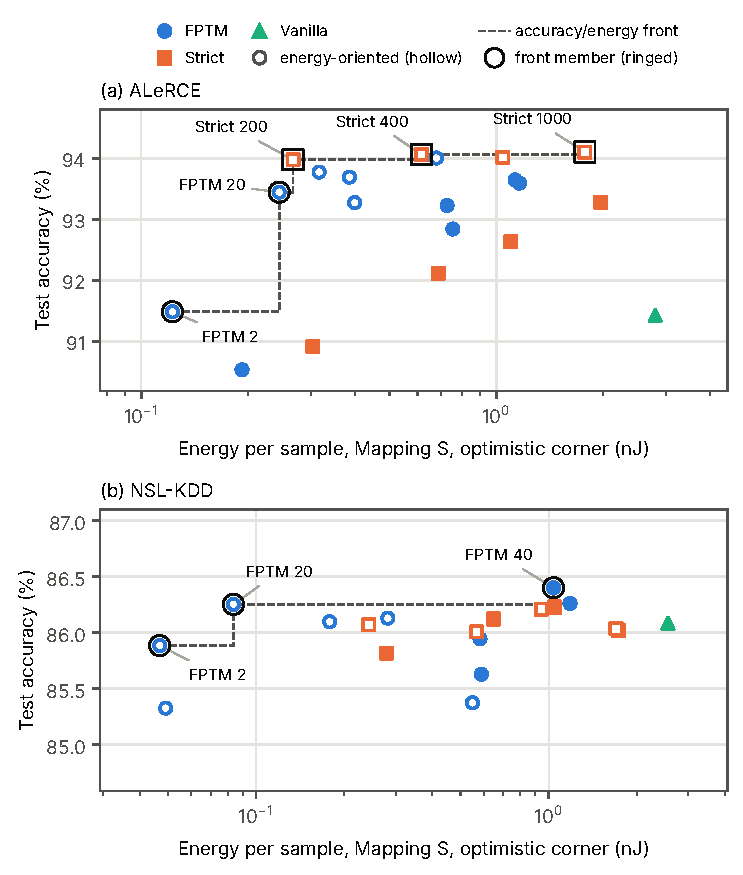
\includegraphics[width=0.92\textwidth]{figures/acc_energy_front.pdf}
\caption{\wosnew{Test accuracy versus predicted Mapping~S energy per sample (optimistic corner) for the accuracy-oriented (filled) and energy-oriented (hollow) hyperparameters. The dashed line is the accuracy and energy front, and ringed points are its members. Unringed points near the line are dominated by less than 0.05 points. Energy includes the controller. The axes are cut to the front region. Below the cut lie the 200-clause vanilla TM of both datasets (78.65\% and 81.22\%) and the accuracy-oriented 2-clause NSL-KDD FPTM (84.11\%).}}
\label{fig:front}
\end{figure}

\paragraph{WOS-46985}\label{sec:wosretune}
\wosnew{On WOS-46985, the two runs differ by at most 0.61 points in accuracy and 32\% in energy.
The energy-oriented FPTM models carry 102 to 607 literals per clause, against 215 to 1,168 with the accuracy-oriented settings. Their predicted energy falls by $2.6\times$ to $25\times$, and their accuracy rises by 0.96 to 3.01 points.
Part of this gain comes from the longer schedule. The 2-clause FPTM, for example, reaches its best validation accuracy only at epochs 239 and 274 of the two runs.}
\wosnew{Even so, the front holds strict models only: the accuracy-oriented and energy-oriented 200-clause models and the energy-oriented 400-clause model.
The cheapest FPTM has 10 clauses per class. It needs 21\% to 23\% more predicted energy than the accuracy-oriented 200-clause strict model} (\hyp{3.77~nJ} and \hyp{1.11~nJ}, 90.87\%). \wosnew{It is also 2.04 points less accurate.
The energy-oriented 200-clause strict model has longer clauses (94 against 74 literals) and needs 13\% to 14\% more predicted energy at the same cycle count.
WOS-46985 is thus the case where FPTM does not pay off on \gainp{}: its text clauses stay long, and long clauses need long miss counts.}

